\begin{frame}{Two-Stage Probability Tree}
\begin{center}
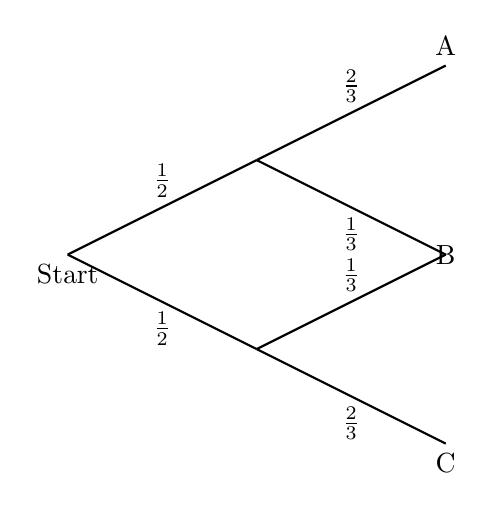
\begin{tikzpicture}[scale=1.2]
    \coordinate (A) at (0,0);
    \coordinate (B) at (2,1);
    \coordinate (C) at (2,-1);
    \coordinate (D) at (4,2);
    \coordinate (E) at (4,0);
    \coordinate (F) at (4,-2);
    
    \draw[thick] (A) -- node[above] {$\frac{1}{2}$} (B);
    \draw[thick] (A) -- node[below] {$\frac{1}{2}$} (C);
    \draw[thick] (B) -- node[above] {$\frac{2}{3}$} (D);
    \draw[thick] (B) -- node[below] {$\frac{1}{3}$} (E);
    \draw[thick] (C) -- node[above] {$\frac{1}{3}$} (E);
    \draw[thick] (C) -- node[below] {$\frac{2}{3}$} (F);
    
    \node[below] at (A) {Start};
    \node[above] at (D) {A};
    \node at (E) {B};
    \node[below] at (F) {C};
\end{tikzpicture}
\end{center}

\footnotesize
Two-stage decision tree with probability labels
\end{frame}